\section{Overview of the System Specification}
% Provide an overview of the initial specification, setting out the main features
% of the system or project and addressing at least system functionality,
% interfaces (electronic and/or human), and signal/information representations. 

Whole system is a plugin for Rodin Platform. It uses translation rules
(\href{http://poporo.uma.pt/docs/rules.pdf}{like this one})
from Event-B to Eiffel and produce Eiffel code. Translation rules has been
provided to me by Victor Rivera. \\

\href{http://wiki.event-b.org/index.php/Plug-in_Tutorial}{Tutorial}
for the extension of the Rodin platform by plugin addition.

Access to plugin functionality will be granted through context menu of specific
machine, like in EventB2Java plugin:\\[2em]
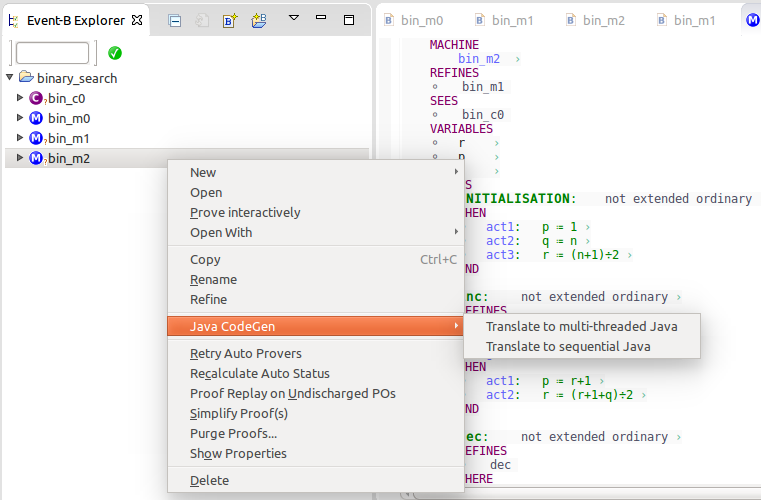
\includegraphics[width=\textwidth]{rodin_plugin}\\[2em]
But in my case it would be \texttt{Eiffel CodeGen} and will translate to Eiffel 
code.\\
